\documentclass{beamer}

\usepackage{txfonts}
\usepackage{hyperref}
\usepackage{fancybox}
\usepackage{xfrac}
\usepackage{cancel}

\newcommand{\heart}{\ensuremath\heartsuit}

\usepackage{mathtools,amssymb}
\newcommand{\myarrow}{\scalebox{2}[2]{$\mathclap{\curvearrowleft}\mkern2.2mu
                                                 \mathclap{\curvearrowright}$}}

\DeclareMathOperator{\Bin}{\mathrm{Bin}}

\hypersetup{colorlinks=false,linkbordercolor=red,linkcolor=green,pdfborderstyle={/S/U/W 1}}

\addtobeamertemplate{navigation symbols}{}{ \hspace{1em}    \usebeamerfont{footline}%
    \insertframenumber / \inserttotalframenumber}

\geometry{papersize={15cm,12cm}}
\usepackage{lipsum}

\makeatletter
\newenvironment<>{contdproof}[1][\proofname]{%
    \par
    \def\insertproofname{#1\@addpunct{.}}%
    \usebeamertemplate{proof begin}#2}
  {\usebeamertemplate{proof end}}
\makeatother


\setbeamertemplate{theorems}[numbered]

\newtheorem{subexample}{Example}

\newtheorem*{nonumdefinition}{Definition}
\newtheorem*{nonumproblem}{Problem}
\newtheorem*{nonumcorollary}{Corollary}
\newtheorem*{nonumproof}{Proof}
\newtheorem*{nonumtheorem}{Theorem}
\newtheorem*{nonumremark}{Remark}
\newtheorem*{answer}{Answer}
\newtheorem*{nonumremarks}{Remarks}
\newtheorem*{nonumexamples}{Examples}
\newtheorem*{nonumsolution}{Solution}
\newtheorem*{nonumexample}{Example}
\newtheorem*{nonumproposition}{Proposition}
\newtheorem{proposition}[theorem]{Proposition}

\usepackage{tikz}
\newcommand*\mycirc[1]{%
  \tikz[baseline=(C.base)]\node[draw,circle,inner sep=.7pt](C) {#1};\:
}

\newcommand\myheading[1]{%
  \par\bigskip
  {\color{blue}{\large #1}}\par\smallskip}

%\usetheme{Warsaw}
%\usetheme{Berkeley} %sample 1

\usetheme{Berlin} % sample 2
%\usetheme{AnnArbor} % sample 3

\let\otp\titlepage
\renewcommand{\titlepage}{\otp\addtocounter{framenumber}{-1}}

\title{Lecture 14 : The Gamma Distribution and its Relatives}
\author{}
\date{}

\begin{document}
\begin{frame}[plain]
\titlepage
\end{frame}

\begin{frame}
The gamma distribution is a continuous distribution depending on two parameters, $\alpha$ and $\beta$. It gives rise to three special cases 
\begin{enumerate}
\item The exponential distribution $(\alpha=1,\beta=\dfrac{1}{\lambda})$

\item The $r$-Erlang distribution $(\alpha=r,\beta=\dfrac{1}{\lambda})$

\item The chi-squared distribution $(\alpha=\dfrac{\nu}{2}, \beta=2)$
\end{enumerate}
\end{frame}

\begin{frame}
\myheading{The Gamma Distribution}

\begin{nonumdefinition}
A continuous random variable $X$ is said to have gamma distribution with parameters $\alpha$ and $\beta$, both positive, if
$$
f(x)=
\left\{
\begin{array}{ll}
\dfrac{1}{\beta^{\alpha}\Gamma(\alpha)}x^{\alpha-1}e^{\sfrac{-x}{\beta}}, & x>0\\
0, & \text{otherwise}
\end{array}
\right.
$$
What is $\Gamma(\alpha)$?

$\Gamma(\alpha)$ is the \underline{gamma function}, one of the most important and common functions in advanced mathematics. If $\alpha$ is a positive integer $n$ then 
$$
\Gamma(n)=(n-1)!
$$
(see page 17)
\end{nonumdefinition}
\end{frame}

\begin{frame}
\begin{nonumdefinition}[Cont.]
So $\Gamma(\alpha)$ is an interpolation of the factorial function \underline{to all real numbers.}

{\large\bf Z} $\lim\limits_{\alpha\to 0}\Gamma(\alpha)=\infty$

\myheading{Graph of $\Gamma(\alpha)$}

\centerline{
\includegraphics{figure/fig1.eps}}
\end{nonumdefinition}
\end{frame}

\begin{frame}
I will say more about the gamma function later. It isn't that important for Stat 400, here it is just a constant chosen so that 
$$
\int\limits^{\infty}_{-\infty}f(x)dx=1
$$
The key point of the gamma distribution is that it is of the form
$$
\text{(constant) (power of $x$) } e^{-cx}, c>0.
$$
The $r$-Erlang distribution from Lecture 13 is almost the most general gamma distribution.
\end{frame}

\begin{frame}
The only special feature here is \underline{that $\alpha$ is a whole number $r$.} 

Also $\beta=\dfrac{1}{\lambda}$ where $\lambda$ is the Poisson constant.

\myheading{Comparison Gamma distribution}
$$
\left(\dfrac{1}{\beta}\right)^{\alpha}\frac{1}{\Gamma(\alpha)}x^{\alpha-1}e^{\sfrac{-x}{\beta}}
$$
\underline{$r$-Erlang distribution} $\alpha=r$, $\beta=\dfrac{1}{\lambda}$
$$
\lambda^{r}\frac{1}{(r-1)!}x^{r-1}e^{-\lambda x}
$$
\end{frame}

\begin{frame}
\begin{nonumproposition}
Suppose $X$ has gamma distribution with parameters $\alpha$ and $\beta$ then
\begin{itemize}
\item[(i)] $E(X)=\alpha\beta$

\item[(ii)] $V(X)=\alpha\beta^{2}$
\end{itemize}
so for the $r$-Erlang distribution
\begin{itemize}
\item[(i)] $E(X)=\dfrac{r}{\lambda}$

\item[(ii)] $V(X)=\dfrac{r}{\lambda^{2}}$
\end{itemize}
\end{nonumproposition}
\end{frame}

\begin{frame}
\begin{nonumproposition}[Cont.]
As in the case of the normal distribution we can compute general gamma probabilities by \underline{standardizing}.
\end{nonumproposition}

\begin{nonumdefinition}
A gamma distribution is said to be standard if $\beta=1$. Hence the $pdf$ of the standard gamma distribution is
$$
f(x)=
\left\{
\begin{array}{ll}
\dfrac{1}{\Gamma(\alpha)}x^{\alpha-1}e^{-x}, & x\geq 0\\
 0, & x<0
\end{array}
\right.
$$
The $cdf$ of the standard
\end{nonumdefinition}
\end{frame}

\begin{frame}
\begin{nonumdefinition}[Cont.]
gamma function is called the \underline{incomplete gamma function} (divided by $\Gamma(\alpha)$)
$$
F(x)=\dfrac{1}{\Gamma(\alpha)}\int\limits^{x}_{0}x^{\alpha-1}e^{-x}dx
$$
(see page 13 for the actual gamma function)

It is tabulated in the text Table A.4 for some (integral values of $\alpha$)
\end{nonumdefinition}

\begin{nonumproposition}
Suppose $X$ has gamma distribution with parameters $\alpha$ and $\beta$. Then $Y=\dfrac{X}{\beta}$ has standard gamma distribution.
\end{nonumproposition}
\end{frame}

\begin{frame}
\begin{proof}
We can prove this, $Y=\dfrac{x}{\beta}$ so $X=\beta y$. 

Now $f_{X}(x)dx=\dfrac{1}{\beta^{\alpha}}\dfrac{1}{\Gamma(\alpha)}x^{\alpha-1}e^{\sfrac{-x}{\beta}}dx$.

\vskip .1cm

Now substitute $x=\beta y$ to get

\smallskip
\centerline{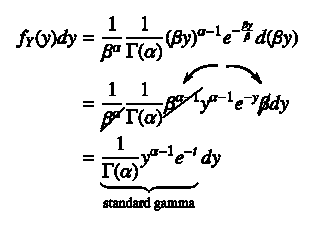
\includegraphics{figure/fig2.eps}}
\end{proof}
\end{frame}

\begin{frame}
%raghu, page 10
\begin{subexample}[4.24 (cut down)]
Suppose $X$ has gamma distribution with parameters $\alpha=8$ and $\beta=15$. Compute 
$$
P(60\leq X\leq 120)
$$
\end{subexample}

\begin{nonumsolution}
Standardize, divide EVERYTHING by $\beta=15$.
\begin{align*}
P(60\leq X\leq 120) &= P\left(\dfrac{60}{15}\leq \dfrac{X}{15}\leq \dfrac{120}{15}\right)\\
                    &= P(4\leq Y\leq 8)=F(8)-F(4)\\
\text{from table A.4} &\\
&= .547-.051=.496
\end{align*}
\end{nonumsolution}
\end{frame}

\begin{frame}

\end{frame}

\begin{frame}

\end{frame}

\begin{frame}

\end{frame}

\begin{frame}

\end{frame}

\begin{frame}

\end{frame}

\begin{frame}

\end{frame}

\begin{frame}

\end{frame}

\begin{frame}

\end{frame}


\end{document}


